\subsection{Review of Motor Identification}

Since the very beginning of the Controller Design phase we realized the necessity of reviewing the results of the \textbf{First Report} dedicated to the Identification of Second Order System (SOS) parameters modelling the \LEGOMOTOR{}. This review was specifically aimed to strengthen our confidence toward the SOS parameters reliability as a starting point for the future work, therefore we conducted further experimentation with new signal filtering approaches that could approximate better approximate the key features of the raw data obtained from the \LEGOMOTOR{}.

In particular we decided to abandon the \textbf{butterworth} filtering technique which introduced heavy delay effects in between the experimental data and the filtered signal, thus leading to a wrong estimation of $\omega_n$. In replacement of butterworth we adopted instead an approach based on \textbf{cubic splines}, a technique used for interpolation. In figure \ref{fig:newfiltering} it is possible to appreciate how the cubic splines allowed us to obtain a filtered signal with a slope nearly overlapping the experimental data, meaning that we are no longer affected by the delay introduced by butterworth and that now our estimate of $\omega_n$ can be more accurate.

\begin{figure}[htbp]
\center
  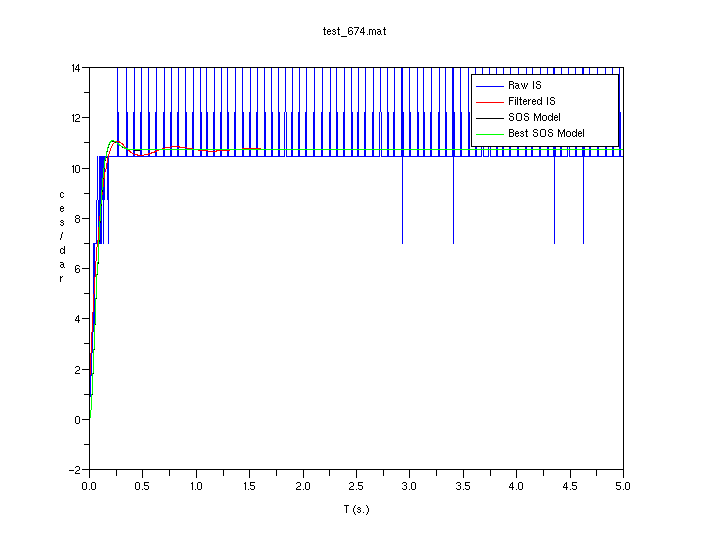
\includegraphics[scale=0.61]{FIGURES_2/power_70_test_24.png}
  \caption[SOSModel]{The response of the system: raw instantaneous speed (blue), filtered signal (red), reconstructed response signal (black) and best SOS model (green).}
  \label{fig:newfiltering}
\end{figure}

Following the same methodology explained in the \textbf{First Report}, we estimated the new SOS parameters of the \LEGOMOTOR{} to be:

\begin{itemize}
	\item $\mathbf{K} = 2.033620$
	\item $\mathbf{\omega_n} = 20.907025$
	\item $\mathbf{\xi} = 0.730782$
\end{itemize}

We should mention that the \textbf{First Report} has been updated accordingly, so that it now displays the newly computed data and graphs.

\subsection{Controller Design}

In this section we will cover the design of a \emph{Controller} for the \LEGOMOTOR{} system with a \textit{Closed Loop System} (CLS), a design architecture in which the output of the system is used as feedback reference for the controller itself.

\subsubsection{Output Signal Acceptable Characteristics}

The first step that has to be taken is to define what are the performance constraints that the output signal produced by the \textit{Closed Loop System} must meet in order to be acceptable for our purposes. Generally speaking we aim to design the system so that it behaves well in the case of input step signals, which means having zero steady state error as well as an early settling time. Therefore the acceptance parameters have been set to:

\begin{itemize}
	\item \textbf{Max Overshoot ($O_{max}$)}: $30\%$
	\item \textbf{Settling Time ($St_{max}$)}: $300 ms$
	\item \textbf{Rise Time ($R_t$)}: $80 ms$
	\item \textbf{Overshoot Time ($O_t$)}: $100 ms$
	\item \textbf{Input Power ($IP$)}: $7.4$ [V]
	\item \textbf{Steady State Value Tolerance ($\alpha{}$)}: $5\%$
\end{itemize}

Recall from the \textbf{First Report} that the \emph{Open Loop System} did not satisfy at all these requirements, in particular it had an average overshoot time of $200 ms$ and settling time of $400 ms$.

Using these parameters as reference one can easily derive the coefficients, namely $\xi$ and $\omega_n$, of the corresponding desired output signal using the following formulas:

	\begin{equation}
  			\xi = {\sqrt{ \log(O_{max})^2 \over \log( O_{max} )^2 + \pi^2 }}
	\end{equation}\label{eq:minCsi}

	\begin{equation}
		\omega{}_{n}^{1} = {{\log(0.05) - \log(\overline{N})} \over {- \xi \cdot St_{max}}}
	\end{equation}
	where \emph{$\overline{N}$} is computed as:$	\overline{N} = \frac{1}{\sqrt[2]{1 - \xi^2}}	$
	
	\begin{equation}
		\omega{}_{n}^{2} = { - \log({(\omega{}_{max} - q) \over (\omega{}_{min} - q) }) \over {\xi \cdot O_t }}
	\end{equation}
	where $ q = k \cdot IP $  and  $\omega{}_{max} = ( O_{max} \cdot q ) + q  $ and $\omega{}_{min} = 0$
	\begin{equation}
		\omega{}_{n}^{3} = {{ 2\cdot{}\pi }\over { 2\cdot{}O_t \cdot \sqrt{1 - \xi^2} } } 
	\end{equation}
	\begin{equation}
		\omega{}_{n}^{4} = { - log(\alpha{}) \over (St_{max} \cdot \xi) } 
	\end{equation}
	
Note that of the several formulas available for $\omega_n$ we decided to adopt the third one, since by plotting the resulting signals we observed it to be the less error prone estimate available.

As a result of these computations we obtain $\omega_n = 33.64$ and $\xi = 0.36$. The corresponding SOS has been plotted and it proved itself to be within our acceptability constraints, since it has a $St_{max} = 230 ms$ and $Ot_{max} = 100 ms$.

Now it is possible to use the couple $(\theta{}, \omega_n)$, where $\theta = asin(\xi) + {pi \over 2}$, on the complex plane to graphically show the region of all parameters that will satisfy our constraints over the signal. Given that by increasing values of $\xi$ both the overshoot and $Rt$ decrease while $St_{max}$ increases, and that by increasing values of $\omega_n$ all the timing parameters ($Rt$, $Ot$ and $St_{max}$) decrease, it follows that the acceptance region is the pink area shown in figure \ref{fig:AcceptanceRegion}. 

\begin{figure}[htbp]
  \begin{center}
  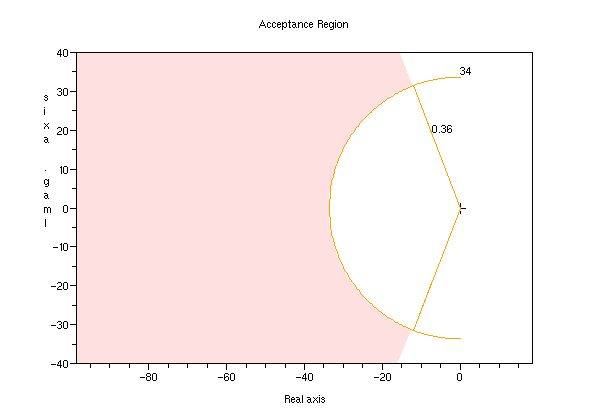
\includegraphics[scale=0.5]{FIGURES_2/AcceptanceRegion.png}
    \caption[Acceptance Region]{The pink area is acceptance region of the SOS system parameters satisfying the imposed constraints}
    \label{fig:AcceptanceRegion}
  \end{center}
\end{figure}

\subsubsection{Root Locus}

The output of the system, considering that for a SISO system $P(s)\cdot{}C(s) = C(s)\cdot{}P(s)$, can be computed as

\begin{equation}
\begin{split}
 Y(s) =& P(s)\cdot{}U(s)\\
 =& P(s)\cdot{}C(s)\cdot{}E(s)\\
 =& P(s)\cdot{}C(s)\cdot{}(R(s)-Y(s))
\end{split}
\end{equation}

hence the \emph{Closed Loop System} transfer function is

\[
Tlf(s) = {{C(s) \cdot P(s)} \over {1 + {( C(s) \cdot P(s) )}}}
\]

where the plant, instantiated with the previously seen parameters, is given by

\[
	P(s) = {{k \over {{s^2 \over {{\omega_n}^2}} + {2s{\xi} \over
        			{\omega_n}} + 1}}U\left (s\right )}
\]


We will determine the transfer function of the Controller so that, when the input signal is a step function, $Y(s)$ meets the acceptance constraints defined in the previous section and, as a consequence, it is stable. This can be done using the \textbf{Root Locus} analysis, a graphical technique that allows to understand how the behaviour of the \emph{Closed Loop System} changes by placing the roots of the \emph{Controller} in different positions of the complex plane.

The first thing to observe in the design of the Controller is that to obtain a zero steady state error with an input step function it is necessary to put a pole in the origin $(0 + 0i)$. More over, in order to attract the Plant poles into the acceptance region we eventually figured out that two complex and conjugated zeros placed at $(-22 + 15i)$ and $(-22 - 15i)$ reach the greatest effectiveness. Finally, to maintain the \textit{causality} of the system and the asymptote more on the left as possible, we put another pole in $(-80 + 0i)$.

As it is possible to see in the figure \ref{fig:RootLocus_CLS}, with the gain of the controller ($kc$) set to $3.5$, we obtain a stable system that respects our acceptance constraints. 

\begin{figure}[H]
  \begin{center}
  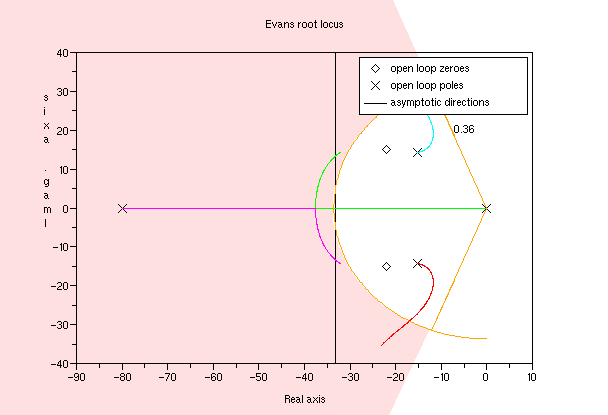
\includegraphics[scale=0.5]{FIGURES_2/RootLocusSinglePoleInZero.png}
    \caption[Root Locus]{Root Locus of the Cloosed Loop System using the designed Controller}
    \label{fig:RootLocus_CLS}
  \end{center}
\end{figure}

The resulting formulas of the Controller is :
\[
		C(s) =3.5\cdot{} {{(s^2 + 44s + 709)} \over {(s^2+80s)}}
\]

\subsection{Analogic Model of the Closed Loop System}

Once the design of the \textbf{Controller} has been established, we need to model our entire system on \textbf{Scicos} to check whether the \CL{}'s performances respect the desired one's as expected.

\begin{figure}[H]
  \begin{center}
  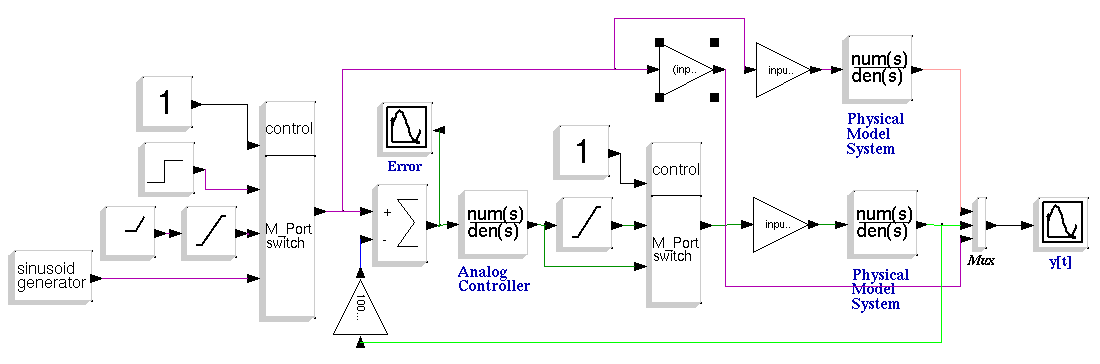
\includegraphics[scale=0.50, angle=90]{FIGURES_2/ScicosAnalogCircuit.png} %width=160mm,height=100mm,
    \caption[Continuous time model]{The Closed Loop System Circuit in the continuous time domain.}
    \label{fig:CT_model}
  \end{center}
\end{figure}

As it is shown in figure \ref{fig:CT_model}, we use an input step function signal for our system. In between the transfer function of the analogical controller and the motor system's transfer function we put a saturation block that accounts for non-linearities and the impossibility of setting the relative speed value of the physical motor outside the interval of values $[-100,100]$ (a typical \emph{windup} phenomenon).

The evolution of the output signal and of the error are shown respectively in figure \ref{fig:analogOutput} and \ref{fig:analogError}.

\begin{figure}[htbp]
  \begin{center}
  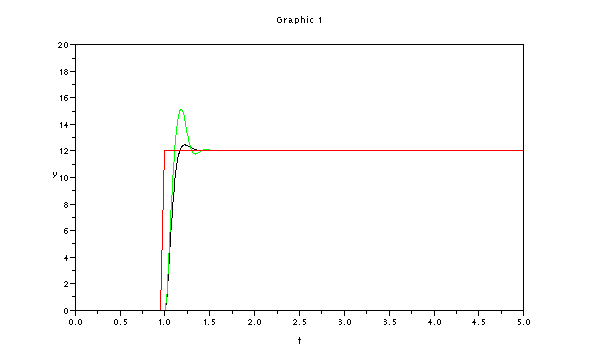
\includegraphics[scale=0.5]{FIGURES_2/CLS-Output-Analog.png}
    \caption[Simulation in Continuous time]{Input Step Signal (red), output signal in with Closed Loop System (green) and output signal with Open Loop System (black).}
    \label{fig:analogOutput}
  \end{center}
\end{figure}

\begin{figure}[htbp]
  \begin{center}
  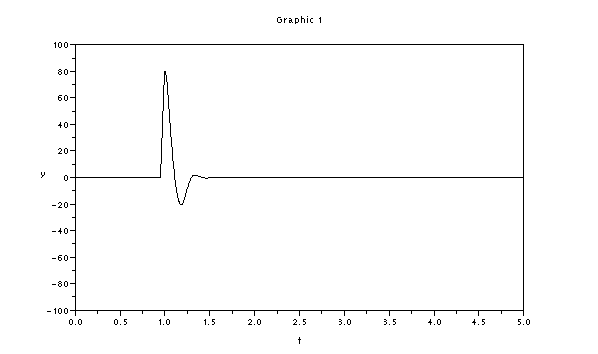
\includegraphics[scale=0.5]{FIGURES_2/CLS-Error-Analog.png}
    \caption[Simulation in Continuous time]{Evolution of the error of the Closed Loop System simulation in continuous time domain.}
    \label{fig:analogError}
  \end{center}
\end{figure}

From the output plots of the continuous time domain simulation we can see that our {\CL} is stable and all the constraints are satisfied because:
\begin{itemize}
	\item the Overshoot comes at nearly $100 ms$ and its peak is not over $30\%$ of the steady state value;
	\item the Error goes to zero as time flows, and the steady state value is stable around the right value;
	\item the Rise time comes at $80 ms$ and the settling time is less than $300 ms$;
\end{itemize}

\subsection{Digital Model of the Closed Loop System}

Once we get in the digital world we need to transform our continuous time Controller into a discrete time Controller, that is substituting the \textit{Laplace} transfer function with the \textit{Zeta-transform} in the \textit{scicos block} of the Controller. One of the easiest and fastest approaches to accomplish this task is to use the \textbf{Bilinear Transform}. This method maps all positions along the $j\omega$ axis, with $Re(s)=0$, of the \textit{s-plane} to the unitary circle of the \textit{z-plane}. Correspondingly, the entire left \textit{s-plane} is mapped within that unitary circle, while the right half \textit{s-plane} is mapped onto the values outside that boundary. Therefore one can easily conclude that a \textit{zeta} transfer function is stable when all its poles are placed within the unitary circle.

Applying the \textbf{Bilinear Transform} is as simple as replacing all occurrences of $s$ with the transform equation
\[
s = {2 \over T}\cdot{}{z-1 \over z+1}
\]

where $T$ is the sampling period, in our case $5 ms$. Applying this transform to the Controller transfer function gives us:
\[
C(z) = 3.5 \cdot{} {(0.7453594 - 1.6592812z + 0.9286927z^2) \over (0.6666667 -1.6666667z + z^2)}
\]

As expected the roots of the denominator fall within the unitary circle: $1$ and $0.6666667$.

To correctly model the behaviour of the \LEGOMOTOR{} we should also take into account the fact that on the brick we can only retrieve estimates of the covered space, which is quantized with $1$ \textit{degree} of precision. Therefore in spite of directly using the output values of the speed at which the motor is running, we should instead derive it from a sequence of quantized covered space estimations. The overall digital circuit is shown in figure \ref{fig:DigitalCircuit}.

\begin{figure}[htbp]
  \begin{center}
  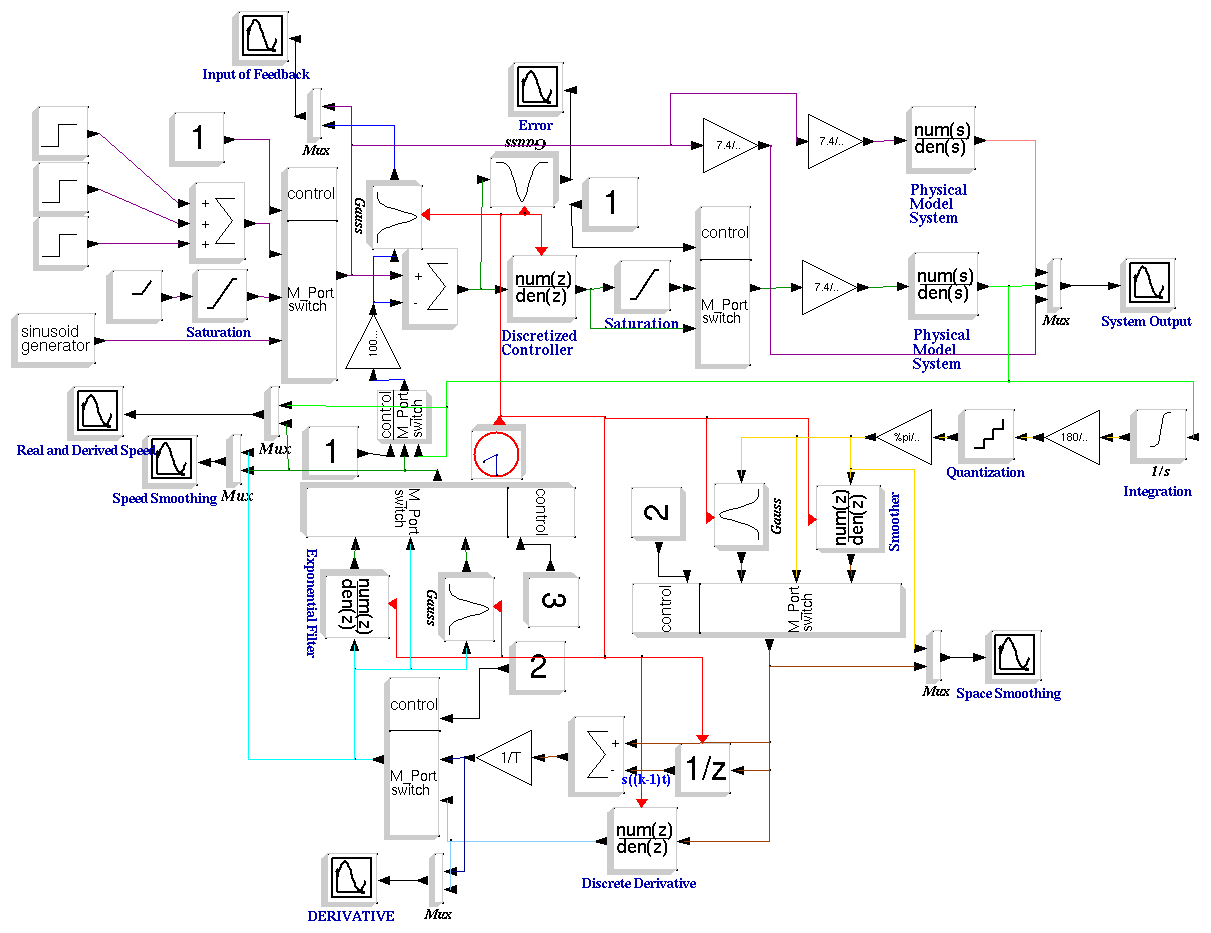
\includegraphics[scale=0.50, angle=90]{FIGURES_2/ScicosDigitalCircuit.png} 
    \caption[Discrete time model]{The Closed Loop System Circuit in the discrete time domain.}
    \label{fig:DigitalCircuit}
  \end{center}
\end{figure}

\begin{figure}[H]
  \begin{center}
  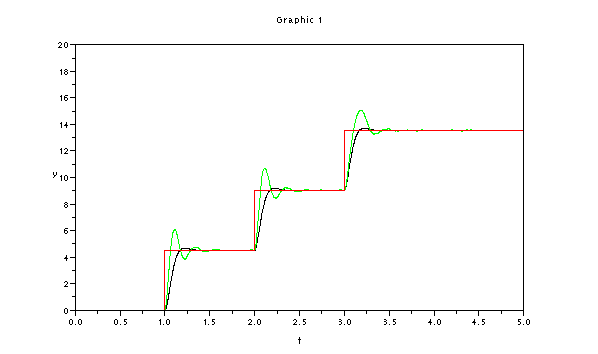
\includegraphics[scale=0.5]{FIGURES_2/CLS-Output-Digital.png}
    \caption[Simulation in Discrete time]{Input Step Signal (red), output signal with Closed Loop System (green) and output signal with Open Loop System (black).}
    \label{fig:digitalOutput}
  \end{center}
\end{figure}

\begin{figure}[htbp]
  \begin{center}
  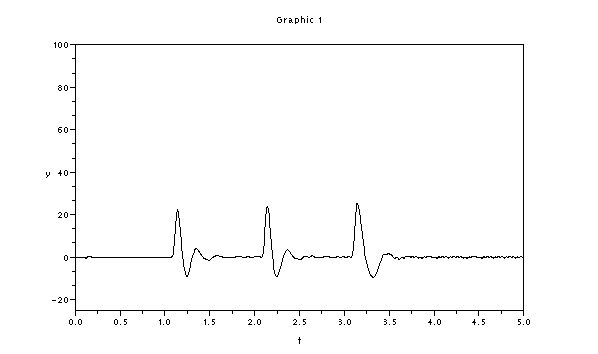
\includegraphics[scale=0.5]{FIGURES_2/CLS-Error-Digital.png}
    \caption[Simulation in Discrete time]{Evolution of the error of the Closed Loop System simulation in discrete time domain.}
    \label{fig:digitalError}
  \end{center}
\end{figure}

The output signal and the error evolution with the digital circuit simulation are shown respectively in figure \ref{fig:digitalOutput} and \ref{fig:digitalError}. Once again, note that the error goes to zero as time lapses and that the output signal is compliant with the imposed requirements as expected.

Note that to achieve the results shown above we had to apply some filtering technique to ensure that noise and spurious results due to the quantization did not affect the reliability of the system. We decided to use the \textit{exponential filter} with forget factor of $0.5$ since it was both effective and simple enough to be implemented. In figure \ref{fig:digitalFilteredSpeed} it is possible to appreciate the improvement gained in the speed estimation by applying the filter.

\begin{figure}[htbp]
  \begin{center}
  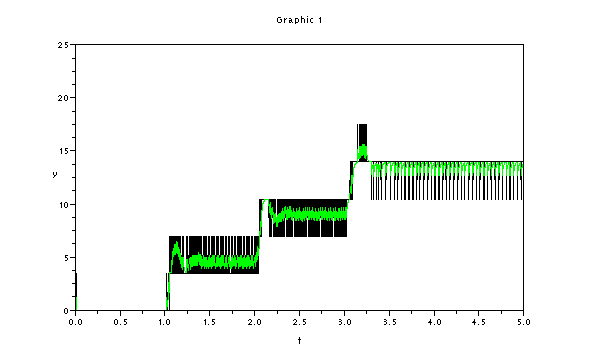
\includegraphics[scale=0.5]{FIGURES_2/CLS-FilteredSpeed-Digital.png}
    \caption[Simulation in Discrete time]{Filtered speed signal (green) obtained from the raw speed values (black) retrieved using the quantized space estimator.}
    \label{fig:digitalFilteredSpeed}
  \end{center}
\end{figure}

%\begin{figure}[htbp]
%  \begin{center}
%  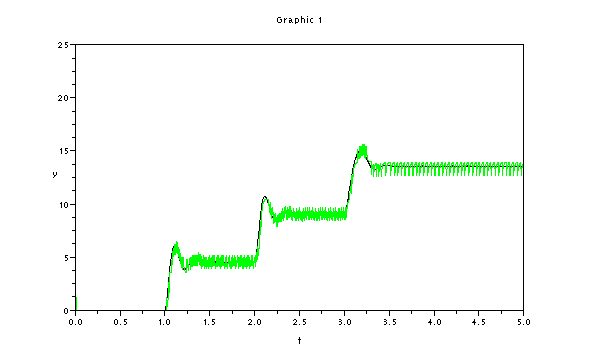
\includegraphics[scale=0.5]{FIGURES_2/CLS-EstimatedSpeed-Digital.png}
%    \caption[Simulation in Discrete time]{Comparison in between the current estimated speed (green) and the real speed at which the system is running (black).}
%    \label{fig:digitalEstimatedSpeed}
%  \end{center}
%\end{figure}

\subsection{\LEGOMOTOR{} Implementation}

The last part of the assignment mandated the development of the controller inside the brick, thus concluding the work previously done on the root locus and the \textit{Scicos} simulations. The discrete controller function implemented on the Brick has been computed  from the \textit{zeta-transform} of the Controller transfer function with the following steps, in which for simplicity the coefficients have been labelled:

\[
\begin{split}
u(k) =&\: kc \cdot{}  {(e_2 + e_1q + e_0q^2) \over (u_2 + u_1q + u_0q^2)} \cdot{} e(k)\\
(u_2 + u_1q + u_0q^2)\cdot{}u(k) =&\: kc \cdot{} (e_2 + e_1q + e_0q^2)\cdot{}e(k)\\
u_2u(k) + u_1u(k)q + u_0u(k)q^2 =&\: kc \cdot{} (e_2e(k) + e_1e(k)q + e_0e(k)q^2)\\
u_2u(k) + u_1u(k+1) + u_0u(k+2) =&\: kc \cdot{} (e_2e(k) + e_1e(k+1) + e_0e(k+2))\\
u(k+2) =&\: {kc \cdot{}(e_2e(k) + e_1e(k+1) + e_0e(k+2)) - u_2u(k) - u_1u(k+1) \over{} u_0}
\end{split}
\]

Since we can not know the future values of the signal, we then applied a change of variable thus obtaining the equation:
\[
u(k) = {kc \cdot{}(e_2e(k-2) + e_1e(k-1) + e_0e(k)) - u_2u(k-2) - u_1u(k-1) \over{} u_0}
\]

For convenience, and coherency with the previous simulations, we decided to transform the angular velocity in the rate of power that can be fed to the motor using a proportional transformation. Part of the code running on the \emph{brick} is shown in the  \emph{C} piece of code below, where you appreciate the simplicity of the control logic that maintains the desired performances for the \LEGOMOTOR{}.

\begin{lstlisting}
// >> CONTROLLER
// Accumulators
float uk_1 = 0;
float uk_2 = 0;
float ek_1 = 0;
float ek_2 = 0;
// Coefficients
float e_2 = 0.7453594;
float e_1 = -1.6592812;
float e_0 = 0.9286927;
float u_2 = 0.6666667;
float u_1 = - 1.6666667;
float u_0 = 1.0;
// KC
float Kc = 3.5;

/**
 * CONTROLLER:
 * Apply the controller computations based on incoming informations
 */
ek_0 = test_target_power - feedback_power_f; // current feedback error
uk_0 = (Kc*((e_2*ek_2)+(e_1*ek_1)+(e_0*ek_0))-(u_2*uk_2)-(u_1*uk_1))/u_0; // current output
ek_2 = ek_1; // Update Discrete Historical values
ek_1 = ek_0;
uk_2 = uk_1;
uk_1 = uk_0;
// Apply Saturation
if (uk_0 > 100)
	uk_0 = 100.0;
if (uk_0 < -100)
	uk_0 = -100.0;

\end{lstlisting}

\subsubsection{\LEGOMOTOR{} execution results}

In order to verify the correctness of our implementation and its capability of respecting the initial constraints, we have done a little of experimentation with our brick.

\subsubsection*{Step Function}
The first experiment consisted into repeating the same kind of analysis that has been done during the \textbf{First Report}. Hence, we have run $50$ tests for all speeds in the power rates interval $[10,100]$, each one distanced by $5$ from the others. We will not show all the graphs and data regarding this analysis here but only the final configuration that our \LEGOMOTOR{} system reaches:

\begin{itemize}
	\item $\mathbf{K} = 2.033363$
	\item $\mathbf{\omega_n} = 26.656639$
	\item $\mathbf{\xi} = 0.625341$
\end{itemize}

The plot \ref{fig:stepTargetPower} shows a typical sequence of power requests that the controller makes to the \LEGOMOTOR{} during a test with an input step function. The high variability of these values could have been decreased by extending the size of the average window that filters the feedback power values, although this would have also introduced a stronger delay in the controller capability of reacting to changes of its input signal.

\begin{figure}[htbp]
  \begin{center}
  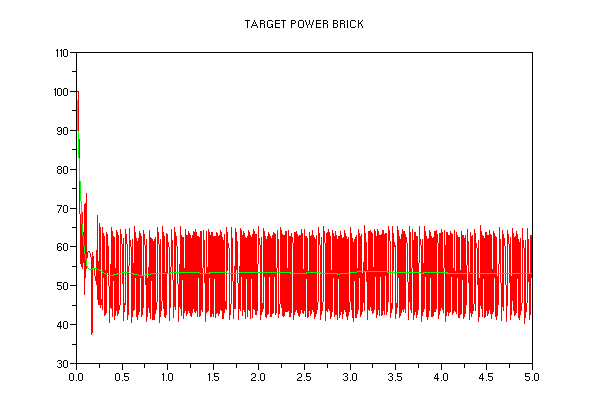
\includegraphics[scale=0.5]{FIGURES_2/BRK-Step-TP.png}
    \caption[]{Controller power response with an input step function of $55\%$.}
    \label{fig:stepTargetPower}
  \end{center}
\end{figure}

The plot of figure \ref{fig:stepFeedbackPower} shows instead the evolution of the feedback power, estimated using the space readings coming from the motor and already filtered. Note that, since the option $brake = ON$ makes the speed of the brick linearly proportional to the input power, this graphs represents also the evolution of the speed of the motor.

\begin{figure}[htpb]
  \begin{center}
  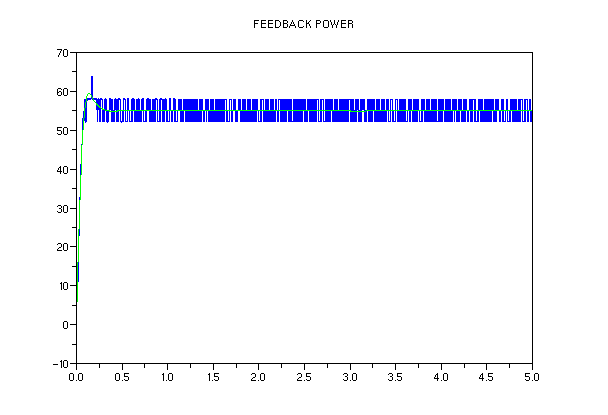
\includegraphics[scale=0.5]{FIGURES_2/BRK-Step-FP.png}
    \caption[]{Feedback power, proportional to the motor speed, with an input step function of $55\%$.}
    \label{fig:stepFeedbackPower}
  \end{center}
\end{figure}

Although the results vary a bit using input step functions of different power level and that the filtering technique applied to the raw speed data introduces some delay in the process, it has been possible to estimate that on average we meet our acceptance constraints: the overshoot is $\leq 30\%$, the $Ts \leq 200 ms$, the $Rt \leq 80 ms$. The only constraint that apparently is not met is the overshoot time $Ot$, that appears to be around $135 ms$ instead of the requested $100 ms$.


A little of delay, around $15 ms$, is to be expected as a consequence of the average filtering technique implemented that slows down the capability of our controller to react to the input values. For the remaining part, this delay should be ascribed to the difficulty of properly filtering and identify the underlying SOS model that characterizes the output signal. This difficulty not only affects the current estimation of the parameters, but it has also affected the results obtained in the \textbf{First Report}. Therefore, it may be due to a slight imprecision in the estimation of the plant's poles that the effectiveness of the Controller is reduced in the real implementation.

After several experimentations with different Root Locus and filtering techniques we could not produce any significant improvement in the overshoot time of the output signal.

\subsubsection*{Step Function with Weight}

We also wished to test our Controller against perturbations induced by the external environment on the motor freedom of rotating. For this reason we have developed an experiment that tests the behaviour of the Controller when one of its motors is repeatedly stressed with an oscillating acceleration. To accomplish this task we took advantage of the earth gravitation force, building ado \emph{LEGO} block made by a couple of gears: one connected to the engine and the other to an external support. Then we attached an off-axis mass to the latter gear, so that the controller would have been forced to increase the motor power during the lift phase and decrease it during the descendant phase. The scheme of this implementation is shown in figure \ref{fig:MotorsModel}.

\begin{figure}[htbp]
  \begin{center}
  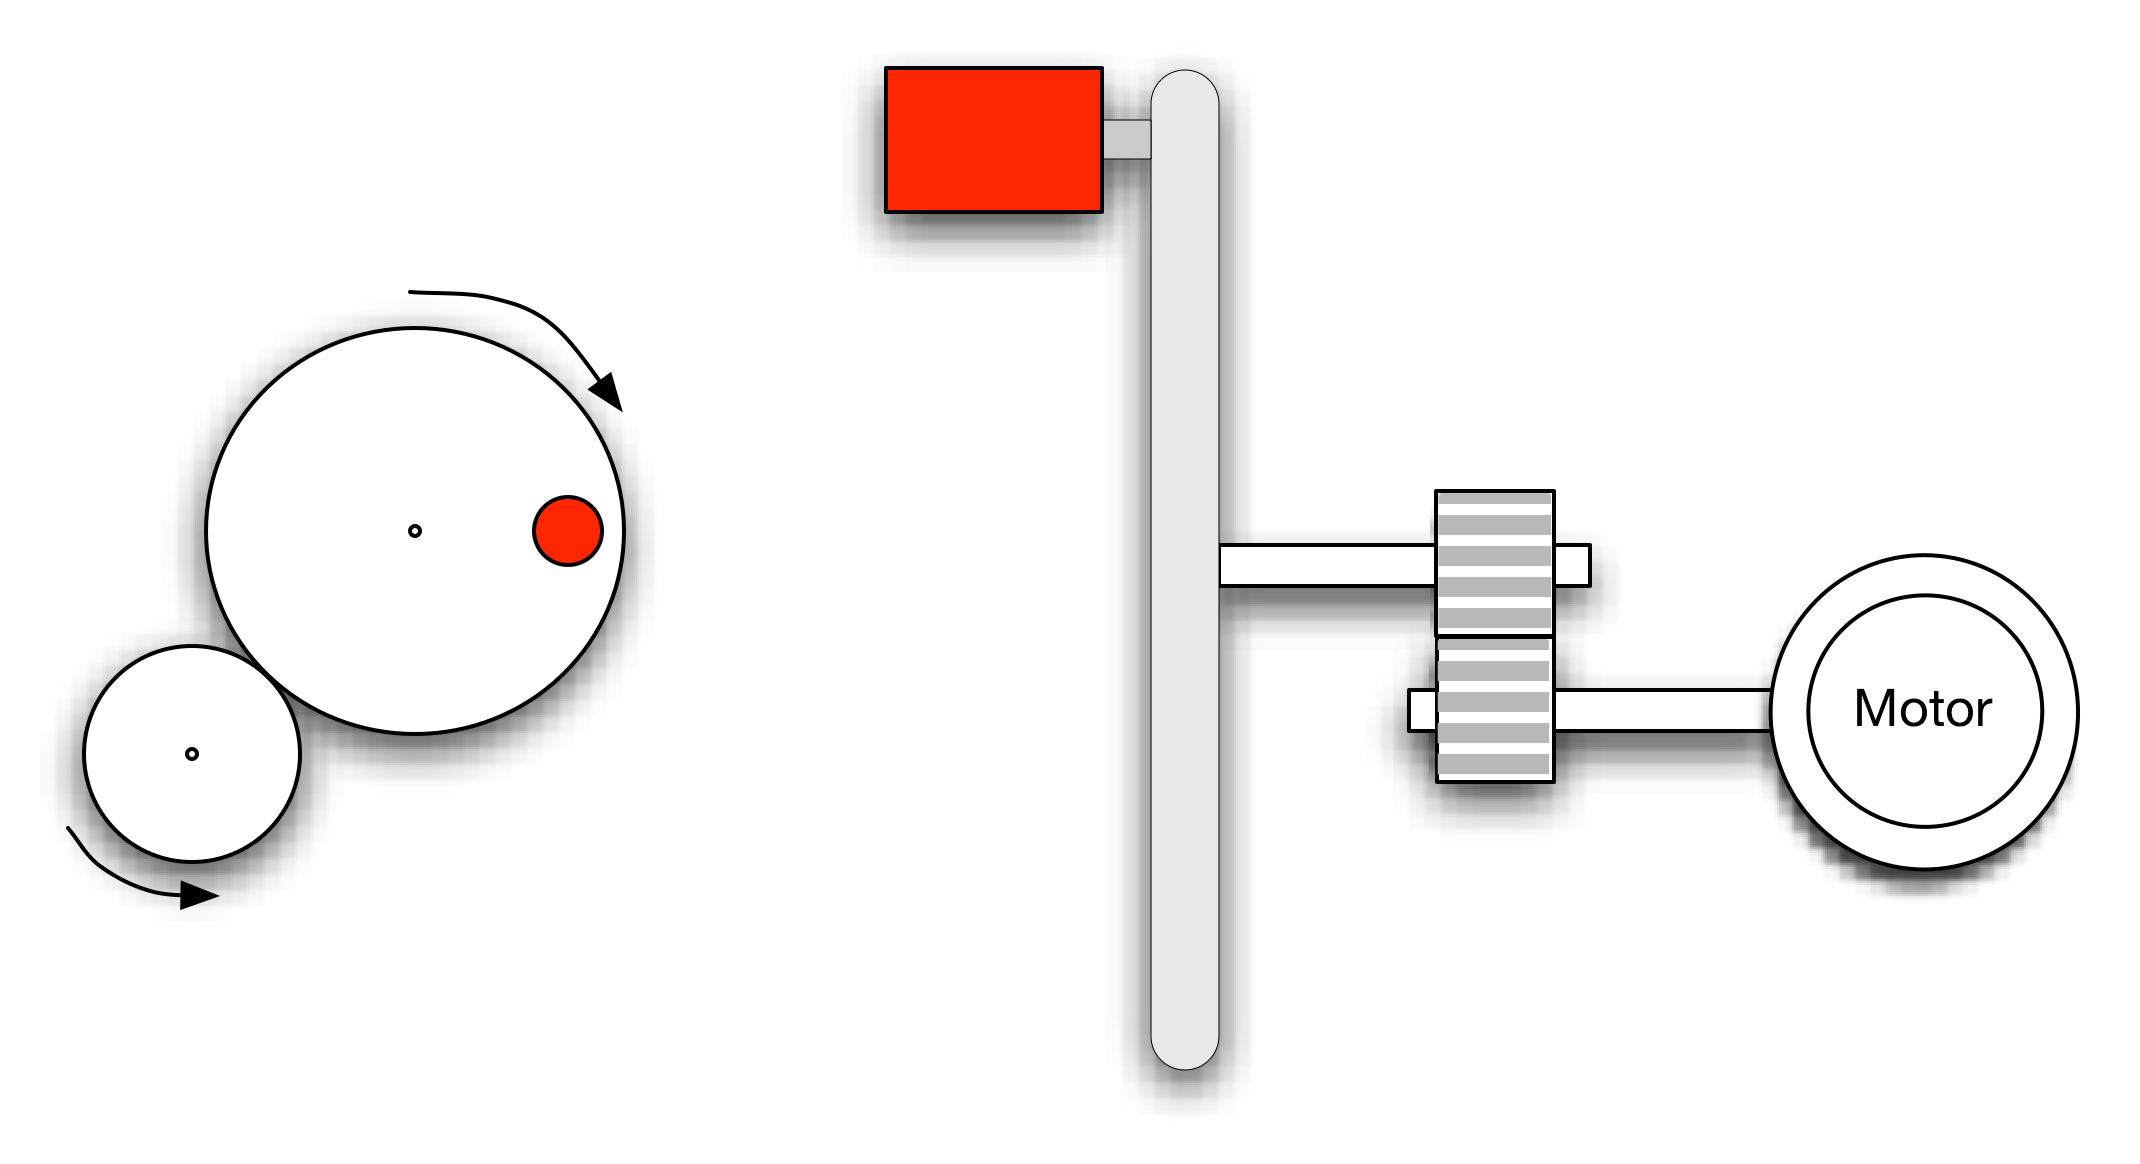
\includegraphics[height=55mm,width=90mm]{FIGURES_2/MotorsModel.png}
    \caption[]{Simple model of the experiment}
    \label{fig:MotorsModel}
  \end{center}
\end{figure}

Although it could have been possible to estimate the gravitational force exerted on the mass and verifying that the resulting acceleration produced by the \emph{Controller} was compliant to our experimental data, due to time constraints we decided to be content with a visual appreciation of the resulting signal. As expected, the controller adjusts the power requests imposed to motor to oppose the sinusoidal acceleration determined by the external environment, as it is shown in figure \ref{fig:weightTargetPower}.  On the converse, despite of the permanent acceleration stress imposed, the speed appears to be stably clanged to the target speed.

Note that this experiment lasted around $30 s$ with samples every $5 ms$, thereby it is natural that these plots appear to be densely populated.

\begin{figure}[H]
  \begin{center}
  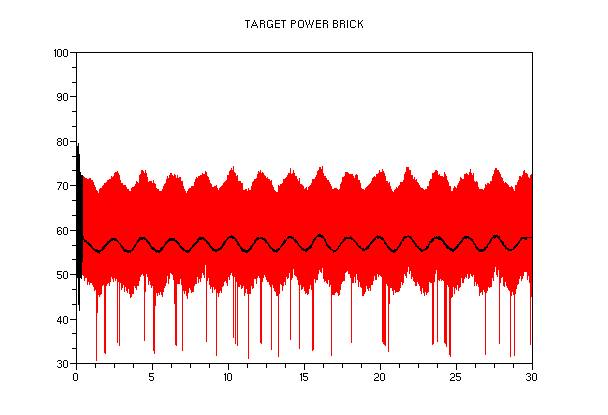
\includegraphics[scale=0.5]{FIGURES_2/BRK-Weight-PR.png}
    \caption[]{Controller power response with a off-axis mass perturbation afecting the motor.}
    \label{fig:weightTargetPower}
  \end{center}
\end{figure}

\begin{figure}[H]
  \begin{center}
  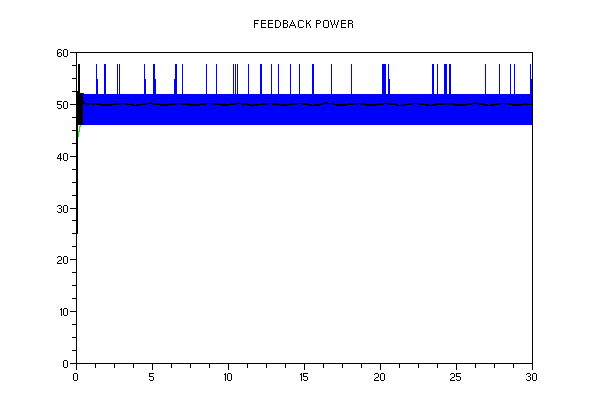
\includegraphics[scale=0.5]{FIGURES_2/BRK-Weight-FP.png}
    \caption[]{Feedback power, proportional to the motor speed, with an off-axis mass perturbation affecting the motor.}
    \label{fig:weightFeedbackPower}
  \end{center}
\end{figure}